%%
%% This is file `./samples/longsample.tex',
%% generated with the docstrip utility.
%%
%% The original source files were:
%%
%% apa7.dtx  (with options: `longsample')
%% ----------------------------------------------------------------------
%% 
%% apa7 - A LaTeX class for formatting documents in compliance with the
%% American Psychological Association's Publication Manual, 7th edition
%% 
%% Copyright (C) 2019 by Daniel A. Weiss <daniel.weiss.led at gmail.com>
%% 
%% This work may be distributed and/or modified under the
%% conditions of the LaTeX Project Public License (LPPL), either
%% version 1.3c of this license or (at your option) any later
%% version.  The latest version of this license is in the file:
%% 
%% http://www.latex-project.org/lppl.txt
%% 
%% Users may freely modify these files without permission, as long as the
%% copyright line and this statement are maintained intact.
%% 
%% This work is not endorsed by, affiliated with, or probably even known
%% by, the American Psychological Association.
%% 
%% ----------------------------------------------------------------------
%% 
\documentclass[man]{apa7}

\usepackage{lipsum}
\usepackage{lscape}

\usepackage[american]{babel}

\usepackage{csquotes}
\usepackage[style=apa,sortcites=true,sorting=nyt,backend=biber]{biblatex}
\DeclareLanguageMapping{american}{american-apa}
\addbibresource{bibliography.bib}

% ellipses (three dots) in quatations definitions from: https://walden-family.com/public/texland/ellipses.pdf
    %dots for main text
    \def\bigdotsspace{3pt}
    %three dots
    \def\mydots{\hbox{\hspace{\bigdotsspace}.\hspace{\bigdotsspace}.\hspace{\bigdotsspace}.\hspace{\bigdotsspace}\hspace{\bigdotsspace}}}
    %I like the same size space on each side of the ellipsis as
    % is between the dots of the ellipsis
    
    \hypersetup{
        nolinks=true,
        colorlinks=false,
        linkcolor=blue,
        filecolor=magenta,      
        urlcolor=cyan,
        pdftitle={Videoconferencing and its Effect on Media Richness Perception, Well-Being and Communication Effectiveness Over Time},
        pdfpagemode=FullScreen,
        % to turn off warning: "Package hyperref Warning: Draft mode on." add empty final attribute
        % final
    }

\title{Videoconferencing and its Effect on Media Richness Perception, Well-Being and Communication Effectiveness Over Time}
% title 2 \title{Changes in Media Richness Perception, Well-Being and Communication Effectiveness in Video-based Communication Over Time}
\shorttitle{Videoconferencing}

\author{Antonio Amaddio}
\affiliation{Freie Universität Berlin \\ A\&O Vertiefung, Winter 2022/23, Supervisor: Dr. Lisa Handke}

\leftheader{Amaddio}

% \abstract{\mbox{}}

\keywords{Media Richness, Compensatory Adaption, Media Naturalness, Channel Expansion, Well-Being, Communication Effectiveness}

%\authornote{
%   \addORCIDlink{Antonio Amaddio}{0000-0000-0000-0000}

  %Correspondence concerning this article should be addressed to Daniel A. Weiss, Department of Educational Psychology, Counseling and
  %Special Education, A University Somewhere, 123 Main St., Oneonta, NY
  %13820.  E-mail: daniel.weiss.led@gmail.com}

\begin{document}
\maketitle
Pandemic related changes in work-life have sparkled a flood of research investigating the psychological effects of remote work. Videoconferencing turns out to be one of the most used communication media to replace a risky face-to-face meeting with a non-risky video based alternative \parencite{Riedl2021}.  Research shares the belief that videoconferencing has a fatiguing psychological effect on its users. The so called \textit{Zoom-Fatigue} seems to be a common reaction to the new media use. The daunting effect is attributed to cue characteristics which are not natural compared to a face-to-face conversation \parencite{Riedl2021}. Our perception has been evolutionary evolved by natural social communication and its cues (verbal, mimic, gesture etc.). If humans are capable to evolve in that sense, why wouldn't humans also adjust to new communication characteristics over time? Therefore, I investigate the experience of one individual in a single case study to explore potential changes in perception and behavior towards videoconferencing over time.

\section{Theoretical Background}

In 1983, \citeauthor{daft1983information} proposed a theory that describes a media’s ability to support communication on a richness scale. That is, how helpful the use of e.g. a telephone is in conveying information required to "reduce uncertainty and clarify ambiguity" (p 5). Media is rated from rich to lean, where Face-to-Face is the richest and numerical formal computer output is lowest in richness. The theory objectively assigns richness to a media. Looking at today’s fully/hybrid remote organizations, where no or only some face-to-face communication is possible, \citeauthor{daft1983information}'s richness categories seem questionable. Given that, teams in these organizations are (1) still functioning and (2) provide enough work for the organization to survive economically.

According to \citeauthor{Kock2005}, this lack of diminished productivity is explained by the workers' effort to compensate for the hindering characteristics of the medium. \citeauthor{Kock2005} suggests that the media barriers increase communication ambiguity and require additional cognitive effort to process relevant pieces of information. He calls workers' behavior to "overcompensate" with lean media information processing: Compensatory Adaption (p. 270). This case study explores factors of ambiguity and factors of increased cognitive effort in video-based communication. It will be operationalized by interviewing the well-being and communication effectiveness of one subject.

The remote workers compensatory adaption effort clearly shapes how they perceive video conferencing's richness initially. It would make sense to assume that remote workers get used to the new way to communicate over time. This means that they might update their appraised richness of video conferencing, by positive/negative experiences with it. Controversy to \citeauthor{daft1983information} the assumptions of \cite{Carlson1999} are adopted.

The authors argue that richness is a personal (subjective) evaluation that one derives from experience. More specifically, experience with the (1) communication partner, (2) channel (media), (3) its topic and the (4) organizational context form a knowledge base. This knowledge can be used to adequately decode information even though the communication media does not naturally support to transfer relevant cues. Similarly, data can be enriched from the sender by encoding information that alleviates understanding by the receiver–which could not be inferred rationally from the raw media message. To summarize: Experience leads to knowledge and shapes the perceived media richness. The question is: how does it do it? The following case study explores which de-/encoding experience has what effect on perceived media richness.

Most studies, finding "Zoom fatigue", have been nomothetic, one-time data collections. This case study confronts generalized characteristics of this effect and explores the underlying changes qualitatively, over time by examining (1) perceived media richness, (2) well-being and (3) communication effectiveness.

\section{Case Study}

The interviewed person is of female sex, 34 years old, married and has one son (17 months). She graduated from a hotel management school, and worked in hotels as a senior convention sales manager. Because of the pandemic crisis and flat hotel booking rates, she moved to a more secure job in a technology start-up 2.5 years ago, where she has been on parental leave for 12 months. The company uses \textit{Gather.town} as its primary video-conferencing tool. She spends 25\% of her time at work communicating in Gather.

The interview took place on 01-30-2023 at 10:30am and lasted $\approx$55 minutes. The interviewee reported preferring face-to-face conversations and to not spend more time than necessary in front of a computer or smartphone. Digital communication in her previous work experience was limited to email and phone. She was selected because she represents an en/decoding expert in natural face-to-face conversations, but a person with a novice-level of videoconferencing skills in a remote work scenario. To relate to the subject, the pseudonym Jane D. will be used.

\subsection{Results}

Baseline for perceived videoconferencing richness was high at the beginning. Jane assumed that videoconferencing shares the same communication characteristics as face-to-face talk. More than that she anticipated, that personal exchange was less overshadowed with commuting distress.

The reported results have been assembled into three tables, separated by each outcome: (1) perceived media richness, (2) well-being, (3) communication effectiveness. The problems of communicating with Gather videoconferencing software have been categorized by its ambiguity (first column). Boxes to the right show related negative experiences (second column), how it was to improved (fourth column) and how it affected the outcome over time (sixth and seventh column). T1 represents the initial rating, T2 the most recent rating.

The activity status in Gather shows if a person is (a) available, (b) busy or (c) doesn't want to be disturbed. In the beginning, Jane often experienced that it was set incorrectly. She reached out to another person–by walking over to the desk virtually–and found no one. After multiple occurrences, she started reacting angrily because of the sloppy behavior of her coworkers (see A, in Box Well-Being on the right). It also effected the teams' communication effectiveness negatively, as she had to find another way to reach out to someone if the activity status has not been updated. She compensated by writing over a chat application (Slack) to the person to get back whenever he/she is really available again. This became the new default route, as the activity status turned out to be most likely wrong. At that point it stopped from effecting well-being and communication effectiveness negatively as this new functional compensation strategy has overcome the dysfunctional experience. However, it reduced her perceived media richness because the activity status turns out to be non-reliable. 

Interestingly, Jane itself did not use the activity status correctly. In Gather one can approach and talk directly to another if the target person has not set the status to "do not disturb". It occurred to her a few times that colleagues directly disturbed her while working when they simply walked over (virtually) and started talking. That verbal interruption was perceived as very obtrusive and left her nervous, anticipating the next obtrusive behavior of a teammate (see B in Figure 1). In most cases a teammate interrupted her regarding a different topic that she was working on. It costed her a lot of energy to cognitively switch the topic or gave a false answer where she had to call back to clarify the mistake afterwards. That shows a negative effect on the communication effectiveness (see T1). She solved that problem by clarifying to anyone that she prefers to be notified first, before someone visits her (virtually) at her desk. This compensation strategy reversed the negative effect on her nervosity level and also the teams communication ineffectiveness (see T2). The dysfunctional experience lead to a sustainable negative effect on her perceived media's richness. She mentioned that in real life, it is common sense to knock on a door before entering a room or visually grab someone's attention instead of "yelling into one's ear". Her explanation shows that updating an activity status does not go offhand naturally. In an office one would see that the target person is either not present on his/her desk, busy talking to another, working in a focussed manner or available to chat. This cue is not given naturally by Gather and is in line with the Media Naturalness Theory of \parencite{Kock2005}.

Another early problem was that the larger the group in a videoconference, the more likely people were to accidentally interrupt each other. She said it was just not obvious who was going to speak next. This was especially true in situations where someone said something humorous where everyone wanted to respond to, verbally. In dyadic conversations, interruptions were most often caused by broadband interference. The latter represented a problem which could not be improved in most cases. The hands were tied when a computer/router reboot did not help. Jane reported, that she also shared the bandwidth of her internet at home with her husband, who also worked remotely. If both used high bandwidth, the video-quality was just about enough to understand colleagues. This lead to less joy when conversing with other people (well-being) as one could not express itself naturally and one had to wait or repeat itself more often because of internet hick-ups. Team members coped with this negative experience by starting to leave longer gaps between conversational turn takings or simply did not react at all. Both strategies were ineffective and left Jane's conversational satisfaction negative. Intriguingly, Jane reported that at the beginning, speaking order confusion lead to communication inefficiency. But as workers started to rule out everything unnecessary from the conversation and talked solely about work related content in a very efficient manner, the effect inversed. The communication became more effective, trading in Joy in conversations. Jane reported that videoconference suggests that everybody could interact at the same time–by looking at everybody's faces at the same time–but fails to transport natural cues where one can deduce who would speak next or simply respond in time with no breaks in between. She mentioned that in a natural setting one would round up around a table where distance between colleagues is given naturally. This kind of sorts out who can interact. This is not given in a we-stare-at-everyones-faces at the same time situation. She reported that this has an acceptable but negative impact on heir perceived richness of videoconferencing. Quite recently, a new team norm where the conversational leader shares a visual board regarding the meetings content reduced speaking-order confusion. Unfortunately, preparing these boards is time-consuming and requires more –videoconferencing caused– extra work.

This result is in line with the overcompensating finding of \citeauthor{Kock2005}'s Compensatory Adaption. Video conferencing introduces an obstacle by this unnatural situation where the video participants try to compensate to have a conversation that is as close as possible to a face-to-face conversation. Jane's willingness to overcompensate is an important motivational constraint \parencite{Kock2001}. Jane has a general expectation that she wants to do a good job. She tackled obstacles introduces by videoconferencing to serve her expectations. Consistently, Jane's work load increased, which she perceived as rather stressful. This shows a negative impact on her well-being over time. That might be different for someone who doesn't have such high standards for themselves.

The last reported problem was ambiguity in emotion expression and appraisal. Jane said that she struggled to take the emotional perspective of her virtual conversational partners. In face-to-face communication, she would rate herself as rather good at recognizing emotions of her counterpart. She said that videoconferencing can not transfer emotions naturally. Further exploration showed that the cause could be attributed to many discrepancies, which sum-up to an incompatibility to read–and express–emotions as she was used to. She reported that it gets harder as the group-size in increases. She reported the following effects on her well-being: She found it fatiguing to scan the amount of faces for emotional expressions. She mentioned that she experienced that coworkers show fewer mimics/gesture at first. Quite probable that teammates were themselves busy scanning everyones faces and the high cognitive load rendered them employed and emotional-expressively blank. Another reported explanation of her was that people are not used to the situation at first, made them nervous and people protected their internal cognitions with external expressive void. Her report shows a negative effect on a workers well-being as the higher cognitive load lead to distress and eventually fatigue (see F in Figure 1). Over time, teammates must have accustomed to the video-setting and coped with a behavior that would be simply unauthentic or exaggerated in face-to-face conversations. People started to express their emotions forming hand gestures like a heart, pointed to their eyes imitating crying, used digital emoticon (=emotion icon) as reactions or verbalized their affections like: "I am overly happy to work within a team like this". Jane perceived this development as rather pleasant. She likes to talk about emotions more openly, which is in line with the team's behavioral change. Over time this reflects a sustainable positive effect on her perceived richness towards videoconferencing regarding emotion expression. She said that it even compensated negative effects on her stress-level and energy-level because she stopped constantly scanning for emotions the old way in video-talks.

The reported results for perceived media richness fit both: (1) the fixed characteristic of the original media richness theory (see \cite{daft1983information}) as well as (2) the individualistic appraisal suggested by Channel Expansion Theory (see \cite{Carlson1999}). Jane's knowledge base of functional behaviors due to her de-/encoding experiences helped her to improve problems introduced by videoconferencing. This affected her appraisal of the media's richness (variability). On the other hand, technical boundaries can not be surpassed fully (fixation). The gap between natural and virtual communication cues can be reduced, but not indefinitely.

\subsection{Conclusion}

Three factors of ambiguity can be concluded from Jane's report in video communication: Activity status, Speaking order and Emotions. Over time, communication ambiguity had a mixed effect on Jane's perceived richness of videoconferencing. Ambiguity regarding the activity status (A) and speaking order (E) could be resolved, with the cost of perceiving videoconferencing as more lean. As Jane herself concluded, this could be due to the fact that this way or another, communicating via video conferencing remains more stressful. May it to transport emotions better or to handle speaking-order.

Quite interestingly, the ambiguity in emotion appraisal, eventually increased her perceived richness of videoconferencing. Despite the extra effort, the coping strategies led to a team-culture that paid more attention to verbalize/react emotionally. The initial problem led to a change in communication that is beyond fixing a technical problem–it enriched the communication quality. It can not be concluded if this is a generalizable positive change, but for Jane, to talk about emotions, to know what is going on in other people is perceived positive.

This case study shows that video conferencing richness is not adequately described by characteristics which generally are assumed to cause "Zoom fatigue". Individual experiences with videoconferencing might vary. This result suggests that either a lot of variables must be controlled or perceived media richness must be studied in a more narrowed down, specific, aspect.

The short observation of three months of Gather usage is a limitation of this case study. A longer period might show other factors and effects of communication ambiguity.

\printbibliography

\appendix

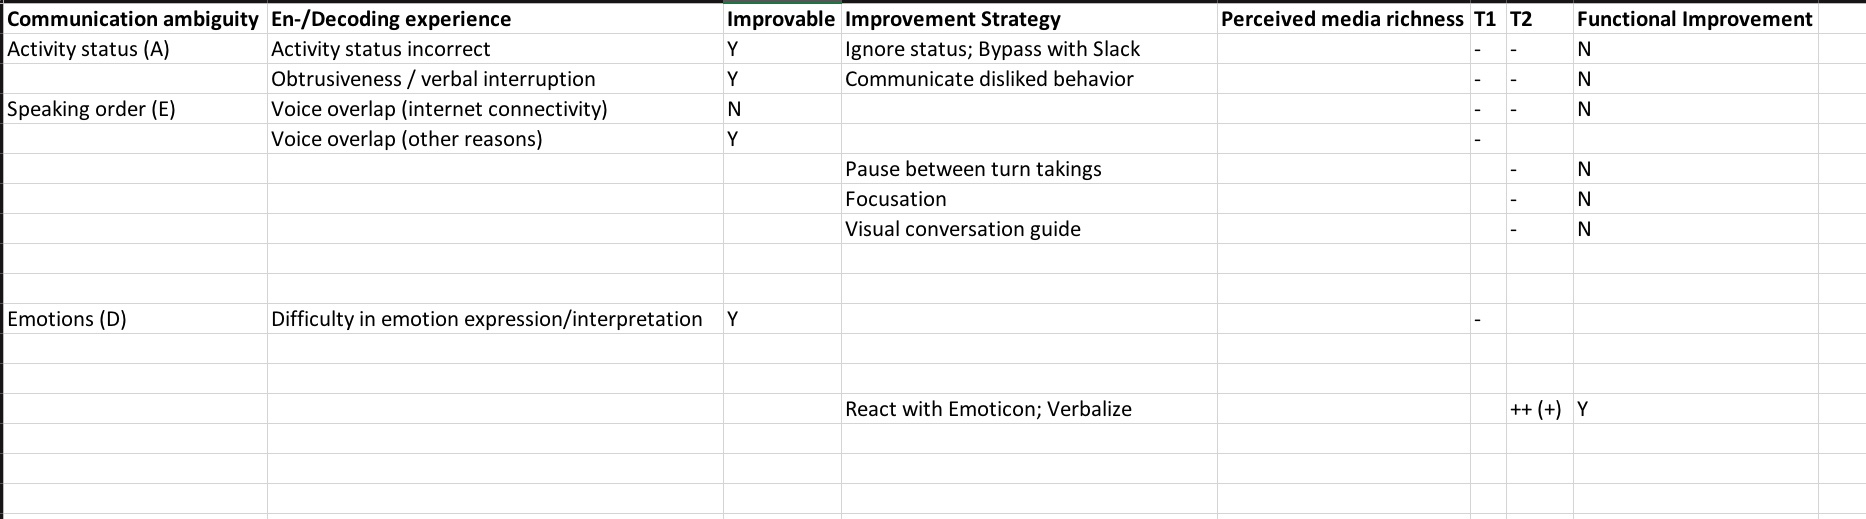
\includegraphics{table-1-perceived-richness.jpg}
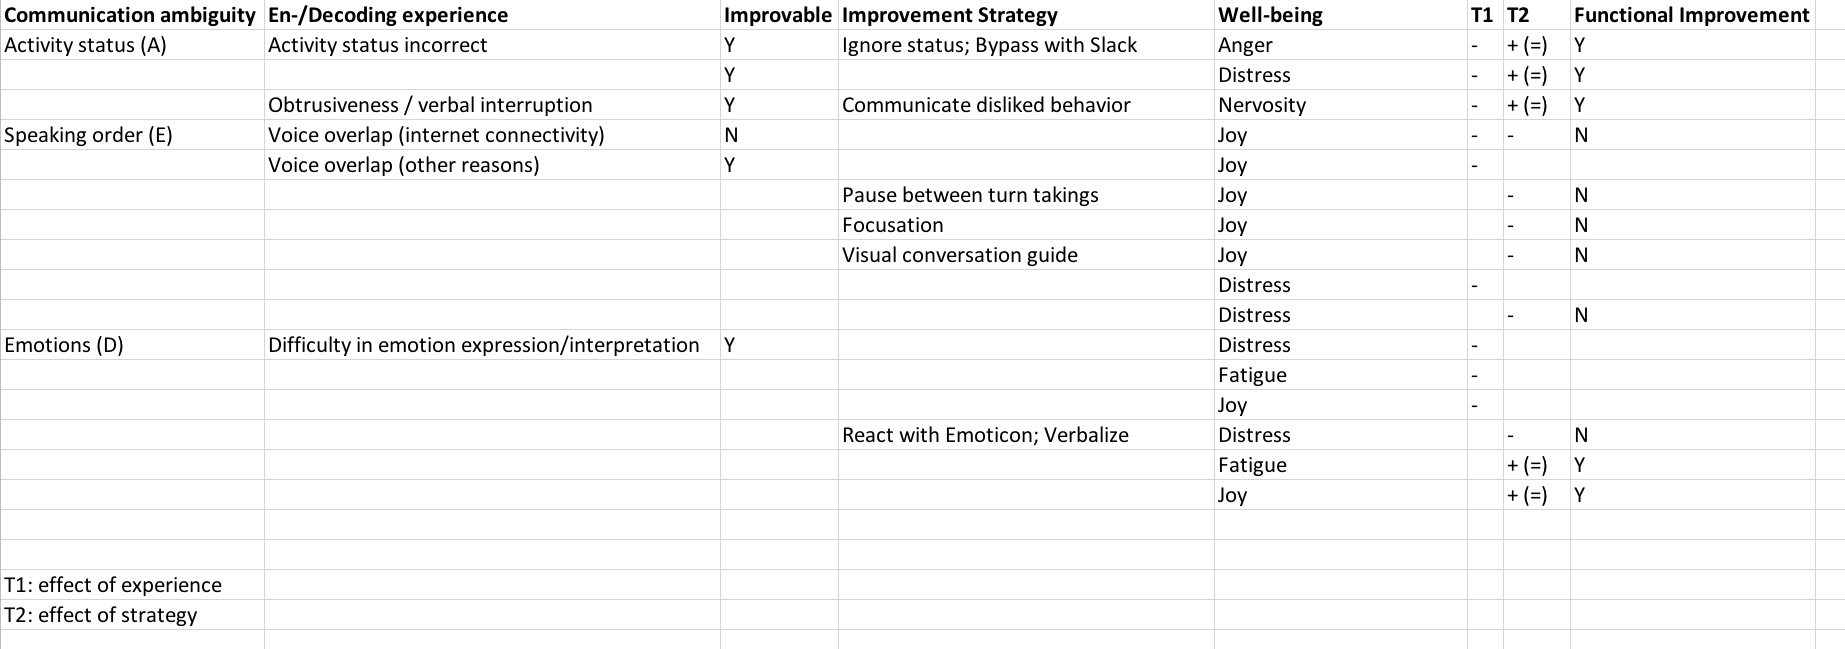
\includegraphics{table-2-well-being.jpg}
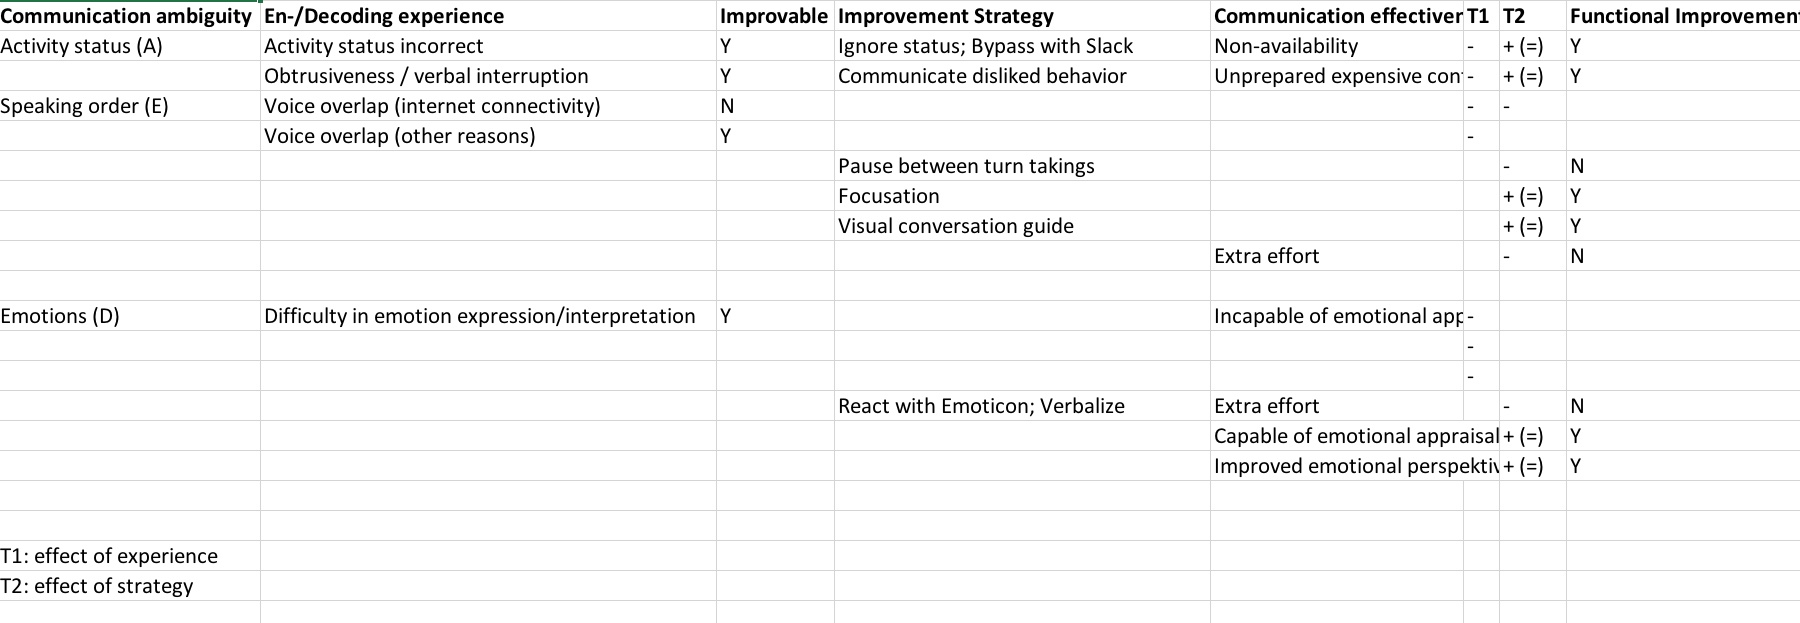
\includegraphics{table-3-comm-effect.jpg}


\begin{landscape}

\begin{table}[]
\begin{tabular}{llllllllllllllll}
\cline{1-5}
\multicolumn{1}{|l|}{\textbf{Communication   ambiguity}} & \multicolumn{1}{l|}{\textbf{En-/Decoding experience}}      & \multicolumn{1}{l|}{\textbf{Improvable}} & \multicolumn{1}{l|}{\textbf{Improvement Strategy}}    & \multicolumn{1}{l|}{\textbf{Perceived media richness}} & \textbf{T1} & \textbf{T2} & \textbf{Functional Improvement} &  &  &  &  &  &  &  &  \\ \cline{1-5}
\multicolumn{1}{|l|}{Activity status (A)}                & \multicolumn{1}{l|}{Activity status incorrect}             & \multicolumn{1}{l|}{Y}                   & \multicolumn{1}{l|}{Ignore status; Bypass with Slack} & \multicolumn{1}{l|}{}                                  & -           & -           & N                               &  &  &  &  &  &  &  &  \\ \cline{1-5}
\multicolumn{1}{|l|}{}                                   & \multicolumn{1}{l|}{Obtrusiveness / verbal interruption}   & \multicolumn{1}{l|}{Y}                   & \multicolumn{1}{l|}{Communicate disliked behavior}    & \multicolumn{1}{l|}{}                                  & -           & -           & N                               &  &  &  &  &  &  &  &  \\ \cline{1-5}
\multicolumn{1}{|l|}{Speaking order (E)}                 & \multicolumn{1}{l|}{Voice overlap (internet connectivity)} & \multicolumn{1}{l|}{N}                   & \multicolumn{1}{l|}{}                                 & \multicolumn{1}{l|}{}                                  & -           & -           & N                               &  &  &  &  &  &  &  &  \\ \cline{1-5}
                                                         & Voice overlap (other reasons)                              & Y                                        &                                                       &                                                        & -           &             &                                 &  &  &  &  &  &  &  &  \\
                                                         &                                                            &                                          & Pause between turn takings                            &                                                        &             & -           & N                               &  &  &  &  &  &  &  &  \\
                                                         &                                                            &                                          & Focusation                                            &                                                        &             & -           & N                               &  &  &  &  &  &  &  &  \\
                                                         &                                                            &                                          & Visual conversation guide                             &                                                        &             & -           & N                               &  &  &  &  &  &  &  &  \\
                                                         &                                                            &                                          &                                                       &                                                        &             &             &                                 &  &  &  &  &  &  &  &  \\
                                                         &                                                            &                                          &                                                       &                                                        &             &             &                                 &  &  &  &  &  &  &  &  \\
Emotions (D)                                             & Difficulty in emotion expression/interpretation            & Y                                        &                                                       &                                                        & -           &             &                                 &  &  &  &  &  &  &  &  \\
                                                         &                                                            &                                          &                                                       &                                                        &             &             &                                 &  &  &  &  &  &  &  &  \\
                                                         &                                                            &                                          &                                                       &                                                        &             &             &                                 &  &  &  &  &  &  &  &  \\
                                                         &                                                            &                                          & React with Emoticon; Verbalize                        &                                                        &             & ++ (+)      & Y                               &  &  &  &  &  &  &  &  \\
                                                         &                                                            &                                          &                                                       &                                                        &             &             &                                 &  &  &  &  &  &  &  &  \\
                                                         &                                                            &                                          &                                                       &                                                        &             &             &                                 &  &  &  &  &  &  &  &  \\
                                                         &                                                            &                                          &                                                       &                                                        &             &             &                                 &  &  &  &  &  &  &  &  \\
                                                         &                                                            &                                          &                                                       &                                                        &             &             &                                 &  &  &  &  &  &  &  &  \\
T1: effect of experience                                 &                                                            &                                          &                                                       &                                                        &             &             &                                 &  &  &  &  &  &  &  &  \\
T2: effect of strategy                                   &                                                            &                                          &                                                       &                                                        &             &             &                                 &  &  &  &  &  &  &  & 
\end{tabular}
\end{table}
\end{landscape}

% \begin{landscape}
% \begin{table}
  % \caption{Impact on Richness Perception, Well-Being and Communication Effectiveness over time}
  % \label{tab:BasicTable}
  % \begin{tabular}{@{}rrrrrrrrrrrrrrrr@{}}         \toprule
                      % &                     &                 &                     &                     &                 & \multicolumn{3}{c}{Lerning rate param}        \\ \cmidrule(r){8-10}
% CA\tabfnm{a}          & EDE\tabfnm{b}                 & I\tabfnm{c} & Improvement Strategy             & Perceived media richness & T1 & T2     & Functional Improvement & Well-being & T1 & T2    & Functional Improvement & Communication effectiveness            & T1 & T2    & Functional Improvement \\ \midrule
% Activity status (A)   & Activity status incorrect     & Y          & Ignore status; Bypass with Slack &                          & -  & -      & N                      & Anger      & -  & + (=) & Y                      & Non-availability                       & -  & + (=) & Y                      \\ 
                      % & Obtrusiveness                 & Y          & Communicate disliked behavior    &                          & -  & -      & N                      & Nervosity  & -  & + (=) & Y                      & Unprepared expensive contextual change & -  & + (=) & Y                      \\ 
% Speaking order (E)    & Voice overlap (inern. connect.) & N          &                                  &                          & -  & -      &                        & Joy        & -  & -     &                        &                                        & -  & -     &                        \\ 
                      % & Voice overlap (other reasons)                              & Y                               &                                                       &                                               & -  &        &                        & Joy        & -  &       &                        &                                        & -  &       &                        \\
                      % &                                                            &                                 & Pause between turn takings                            &                                               &    & -      & N                      & Joy        &    & -     & N                      &                                        &    & -     & N                      \\
                      % &                                                            &                                 & Focusation                                            &                                               &    & -      & N                      & Joy        &    & -     & N                      &                                        &    & + (=) & Y                      \\
                      % &                                                            &                                 & Visual conversation guide                             &                                               &    & -      & N                      & Joy        &    & -     & N                      &                                        &    & + (=) & Y                      \\
                      % &                                                            &                                 &                                                       &                                               &    &        &                        & Distress   &    & -     & N                      & Extra effort                           &    & -     & N                      \\
% Emotions (D)          & Difficulty in emotion expression/interpretation            & Y                               &                                                       &                                               & -  &        &                        & Distress   & -  &       &                        & Incapable of emotional appraisal       & -  &       &                        \\
                      % &                                                            &                                 &                                                       &                                               &    &        &                        & Fatigue    & -  &       &                        &                                        & -  &       &                        \\
                      % &                                                            &                                 &                                                       &                                               &    &        &                        & Joy        & -  &       &                        &                                        & -  &       &                        \\
                      % &                                                            &                                 & React with Emoticon; Verbalize                        &                                               &    & ++ (+) & Y                      & Distress   &    & -     &                        & Extra effort                           &    & -     & N                      \\
                      % &                                                            &                                 &                                                       &                                               &    &        &                        & Fatigue    &    & + (=) &                        & Capable of emotional appraisal         &    & + (=) & Y                      \\
                      % &                                                            &                                 &                                                       &                                               &    &        &                        & Joy        &    & + (=) &                        & Improved emotional perspektive taking  &    & + (=) & Y                     
% \end{tabular}
  % \begin{tablenotes}[para,flushleft]
        % {\small
            % \textit{Note.} Some combinations are duplicate but listed for full comprehension.
% 
            % \tabfnt{a}Instructed finger to move.
            % \tabfnt{b}The finger that has actually been moved.
            % \tabfnt{c}The finger the subject observes in 3D goggles which moves.
            % \tabfnt{d}Motor error.
            % \tabfnt{e}Feedback error.
            % \tabfnt{f}Activation in extrastriate body area.
            % \tabfnt{g}Learning rate parameter according to \textit{resilient} rule.
            % \tabfnt{h}Learning rate parameter according to \textit{hinderance} rule.
            % \tabfnt{i}Learning rate parameter according to \textit{overwrite} rule. Learning rates divided by 10 fingers, to simulate individual learning each finger. A positive/negative value means beneficial/detrimental directed learning, zero means no learning.
            % The letter \textit{A} represents any possible finger, \textit{B} represents any possible finger other than \textit{A}.
         % }
    % \end{tablenotes}
% \end{table}
% 
% \end{landscape}
\end{document}

%% 
%% Copyright (C) 2019 by Daniel A. Weiss <daniel.weiss.led at gmail.com>
%% 
%% This work may be distributed and/or modified under the
%% conditions of the LaTeX Project Public License (LPPL), either
%% version 1.3c of this license or (at your option) any later
%% version.  The latest version of this license is in the file:
%% 
%% http://www.latex-project.org/lppl.txt
%% 
%% Users may freely modify these files without permission, as long as the
%% copyright line and this statement are maintained intact.
%% 
%% This work is not endorsed by, affiliated with, or probably even known
%% by, the American Psychological Association.
%% 
%% This work is "maintained" (as per LPPL maintenance status) by
%% Daniel A. Weiss.
%% 
%% This work consists of the file  apa7.dtx
%% and the derived files           apa7.ins,
%%                                 apa7.cls,
%%                                 apa7.pdf,
%%                                 README,
%%                                 APA7american.txt,
%%                                 APA7british.txt,
%%                                 APA7dutch.txt,
%%                                 APA7english.txt,
%%                                 APA7german.txt,
%%                                 APA7ngerman.txt,
%%                                 APA7greek.txt,
%%                                 APA7czech.txt,
%%                                 APA7turkish.txt,
%%                                 APA7endfloat.cfg,
%%                                 Figure1.pdf,
%%                                 shortsample.tex,
%%                                 longsample.tex, and
%%                                 bibliography.bib.
%% 
%%
%% End of file `./samples/longsample.tex'.
